\documentclass[11pt]{article}
\usepackage{graphicx}
\usepackage[utf8]{inputenc}
\usepackage{amsmath}
\usepackage{gensymb}
\usepackage{setspace}
\usepackage{caption}
\usepackage{subcaption}
\usepackage{wrapfig}
\usepackage{caption}
\usepackage{csvsimple}
\usepackage[font=scriptsize,labelfont=bf]{caption}
\usepackage{csvsimple}
\usepackage{amssymb}
\usepackage[title]{appendix}
\usepackage{textgreek}
\usepackage{amsmath}
\usepackage{harvard}
\usepackage{parskip}
\usepackage[a4paper,width=160mm,top=20mm,bottom=20mm,bindingoffset=6mm]{geometry}
\usepackage{fancyhdr}
\pagestyle{fancy}
\fancyhead{}


\linespread{1.25}

\begin{document}

\begin{titlepage}
    \begin{center}
    \vspace*{1cm}

    \Huge
    \textbf{\underline{Modelling the effects of Gene Flow and Selection on the Canalisation}}\\
    \textbf{\underline{of an established Genetic Network}}\\

    \vspace*{2.0cm}

    \large
    \textbf{Author: Matthew Campos}\\
    \textbf{Submitted August 2020}

    \vspace*{0.8cm}

    \normalsize
    A thesis submitted in partial fulfilment of the requirements for the degree of Master of Science/Research at Imperial College London\\
    Formatted in the journal style of Evolution \& Development\\
    Submitted for the MSc in Computational Methods in Ecology and Evolution\\

    \vspace*{0.8cm}

    \end{center}
\end{titlepage}


\newpage

\section{Declaration}
All raw data collected were from the simulation I created for my project. The simulation requires the input of genetic model systems, and mathematical equations used to derive output. The model system and equations used in the simulation were sourced from the work of \textit{Omholt et al} (2000) and \textit{Gjuvsland et al} (2007). I was reponsible for data processing, cleaning and analysis. All analyses presented in the paper are from the simulations, with the help of my supervisor.

\section{Acknowledgements}
I would like to firstly thank Dr. Scott Rifkin for being a wonderful supervisor and guiding me throughout the project. This includes understanding background knowledge, results and overall research purposes. Secondly, thank you to Dr. Thomas Bell for agreeing to be my internal supervisor, making sure I am aware of the process of the project and ensuring my safety during such difficult times. Also to Dr. Samraat Pawar and Dr. James Rosindell for co-leading a challenging but rewarding CMEE course.
\\Finally I would like to thank the laboratory of Dr. Rifkin- Antonia Darragh, Jessica Bloom, Alexis Cugini, Yang Bing and Rachel Goodridge for being very welcoming and having wonderful and insightful weekly meetings. Good luck with everything!

\newpage

\section{Abstract}
Studies have shown how the role of genotypic evolution on phenotype. How simple alterations in the pathways can lead to pronounced differences in species morphology. Using the genetic model of \textit{Omholt et al}(2000) and \textit{Gjuvsland et al}(2007), I investigate the interplay between gene flow and adaptive processes in the development of a genetic network showing a balance between selection, a strong driver towards canalisation of the network, and gene flow which attempts to homogenise the populations, with the expectation that long temporal periods of evolution with gene flow should lead to a more canalised network compared to without gene flow. Canalisation is represented by fitness values, which are determined by trait values. Heterozygosity in the population has been shown to drive fitness and quickly lead to canalisation while homogeneity relies on chance beneficial mutations, recombination or migrant allele values to become robust. The results show a possible effect that migratory pattern has on the canalisation of a network, and how it is network development could be context dependent. Outcomes from this study can be used to better understand phenotype-genotype relationships and the patterns that drive the development of species.

\newpage

\section{Introduction}
% ITEX root = ../thesis.tex
Species migration can result in the following: (i) it allows individuals and species to colonise new areas and create new subpopulations. Over time, ecological events cause species to become reproductively isolated. This is known as allopatric speciation and it leads to the splitting of lineages, differentiating both related populations long-term. This differentiation also increases with geographic distance. Without gene flow, both sets of species are able to rapidly evolve in their local optimums /cite{garcia1997genetic}. Overall, species that are reproductively isolated have more pronounced modifications which can be observed phenotypically and genotypically \cite{pongratz2002genetic,sato2006effect}. (ii) Migration can allow isolated species to attempt to colonise each other’s habitats. If species are capable of interbreeding, parapatric or peripatric speciation may occur, depending on distance. This introduces new sets of alleles into an environment and as species interact and pass on its heritable genes, it changes the developing genetic makeup of local species. The latter case includes gene flow which helps to maintain the genetic diversity in an area but has been shown to homogenize populations over long periods of time, through the recombination of genes \cite{sato2006effect}. Advancements in genotypic techniques now enable us to study the genotypic effects and further our understanding of phenotype-genotype relationship. As organisms evolve, phenotypic evolution is assisted with genotypic evolution. Collective expression of certain genes through pathways assist in the morphology and behaviour we observe in species. Hereditary genome alterations through random changes in molecular mechanisms change varying aspects of the species \cite{chandrasekaran2008origins} These molecular changes induced by mutation and recombination lead to the variation of descending species \cite{chandrasekaran2008origins,ohno1999gene,brown2002genomes}. Over time, evolutionary forces involving drift and selection acts on these polymorphisms and those most fit passes their variant genome, and phenotype as a result to future generations. This is the foundation of Darwin’s theory natural selection.
\\To better understand species evolution, we can focus on the development of their genome network. Orr showed that there is variation with respect to genetic differences or gene influence on phenotype. The effects of adaptive and non-adaptive processes vary among species where there is no common set of genes involved, nor is the effects and interactions of the genes similar for species \cite{orr1998population} Although generalizations cannot be made of genetic function and interactions, what can be considered is the pattern at which these genetic processes develop over time. Genetic network simulations can be used to understand these patterns of evolution and the effect on phenotype-genotype relationships. Long temporal periods allow genetic interactions within a network to robustly develop, canalising the network \cite{orr1998population,lynch2007evolution}. Lynch highlighted the significance of non-adaptive processes as well in shaping genetic networks. His study showed that networks can still evolve its architecture and become redundant even without the influence of natural selection \cite{lynch2007evolution}. Robustness can evolve from the effects of epistasis, additivity and dominance, all of which are connected \cite{omholt2000gene}.
\\Species evolution is non-linear, descending with modification and constant splitting from lineages of a common ancestor. This continuous process over long temporal periods results in the accumulation of optimal genetic adaptations that results in a robust network structure. This can be quantified through fitness or reproductive success. There is a balancing act as selection aids to propagate fitter variants in a population, while mutation and environmental change limits such propagation \cite{burt1995evolution}. What this study focuses on is how these forces affect the development of genes and the genetic network. Specifically, with the effects of gene flow on a genetic network that has evolved in isolation. The patterns of change that a genetic network undergoes with these adaptive and non-adaptive evolution processes. Even once a robust structure is reached, how does the structure resist change and maintain its network despite perturbations and evolutionary processes. As species evolve, studies have shown that pathways have a safety margin, that make them resistant to change such as mutations \cite{bourguet1999evolution}. Species best suited to their environment will evolve to their local optima, which we can represent as a quantitative value. The further apart these values are, what I label as environmental distance, the greater the variance of the two species. The concern is on how a network responds when these evolutionary forces come into play and seeing the evolving genetic interactions. Investigating the effects of changing migration rates, two variant genetic networks, environmental distance and patterns of migration.
\\Ecological events eliminate barriers and allow species to migrate into new environments, introducing new sets of genes in an environment. The presence of variant genes and network structures from gene flow hinders local adaptation and fixation of adaptive genes \cite{burt1995evolution}. Using quantitative trait loci (QTL) we are able to numerically interpret and visualise the patterns of change. Previous research looked at the effects of gene flow, selection and mutation at generating local adaptation at the phenotypic level, showing how maintenance of alleles and linkage is important in adaptation \cite{yeaman2011genetic}. It was shown that with random perturbations and aid of genetic modifiers, there are bounds for which selection for canalization can act on, leading to evolution of robustness. They also showed that under migration selection balance, selection for robustness increases with the migration rates \cite{proulx2005opportunity}. This research will be looking at the changes in genetic architecture dynamics and the interactions of the varying systems. As a genetic network evolves, there exists a threshold which is actively regulating these homeostatic genes \cite{gjuvsland2007threshold}. As selection for robustness occurs within the local population, it can give insight into the change in architecture and statistically significant interaction \cite{gjuvsland2007statistical}.
\\Using a multi-locus system, I will construct a genetic network and simulate the effects over many generations and see how the output of the network changes, specifically looking at allelic interactions and tracking the fitness over time. Variance in fitness should decrease as a genetic network becomes robust, making it resistant to perturbations. Fitness can be quantified as reproductive success and is represented by passing on quantitative values generated from the alleles. These values are used to derive the trait values of individuals of which phenotypic values are then calculated and used as probabilities for fitness. The expectation is that after migration, a more robust network is formed when compared to before migration. At the start allowing new alleles to enter the population will result in a less robust network and more susceptible to perturbations \cite{garcia1997genetic}. Especially when the migrant network is a different structure, gene flow will allow maladaptive alleles to enter and should those be passed on, will impose a fitness cost to individuals \cite{tigano2016genomics} However, over time, the network should adapt and become resistant to such perturbations.


\newpage

\section{Methods}
% ITEX root = ../Campos_Matthew_CMEE_2020.tex
I wrote a R script that constructs a genetic network, and a variant form, and simulates its evolutions, allowing migration to occur between two populations. All functions to perform adaptive and non-adaptive processes were written from scratch and implemented in the simulation. The following functions are:
\begin{itemize}
    \item Population: initialises the starting populations of specified size where each individual (row) contains 12 allele sites (4 per gene). Since it is a di-allelic model, it is a 2-dimensional array.
    \item Fitness: determines the fitness value of each individual based on their trait values and used as a probability for offspring contribution. A heavy tailed Cauchy distribution is used to determine fitness value from trait values. Each individual has a probability of passing on their genotype to the next generation and function randomly samples from the distribution to select parents, representative of genetic drift.
    \item Mutation: produces an array same dimensions as the population and random uniformly distribution of values to determine which sites undergo mutation based on inputted mutation rate. Generates a new value using a normal function with current value as the mean and a standard deviation of 0.001.
    \item Recombination: randomly chooses which site, and if any consecutive sites downstream, to switch allele values for each individual.
    \item Migration: using a uniform distribution, randomly generates values for each individual in the migrant population to determine which individuals will migrate and replace those in the main population. Population is kept constant in both populations, representing a balanced dispersal between immigration and emigration \cite{rice2009evolution,w2004dispersal}.
\end{itemize}
\subsection{The model}
A di-allelic interlocus model from the research of \textit{Omholt (2000)}. In this case, all the genes are hereditary, representing only the regulatory and coding region which determine protein expression and rate of expression. Studies has shown that mutations along the coding region are known to cause morphological variation within species \cite{stern2009genetic}. This model structure evolves dominance through epistatic interactions and autoregulatory effects. Using a system of equilibrium solutions and solved ordinary differential equations (ODE), simulated protein concentrations corresponding to phenotype are measured over time \cite{omholt2000gene}. Here I consider the loci as quantitative factors of protein function, and trait value is determined by protein concentrations. The greater the amount of protein expressed, the larger the trait value. The model consists of three genes, $X_1$, $X_2$ and $X_3$. Let \(j\) represent the genes where $j = {1,2,3}$, each gene $X_j$ consists of two alleles, $X_{j1}$ and $X_{j2}$. This leads to the formula:
\begin{equation*}
    y_j = X_{j1}  + X_{j2} \label{eq:Protein Expression} \tag{1}
\end{equation*}
\begin{wrapfigure}{l} {0.7\textwidth}
    \begin{center}
        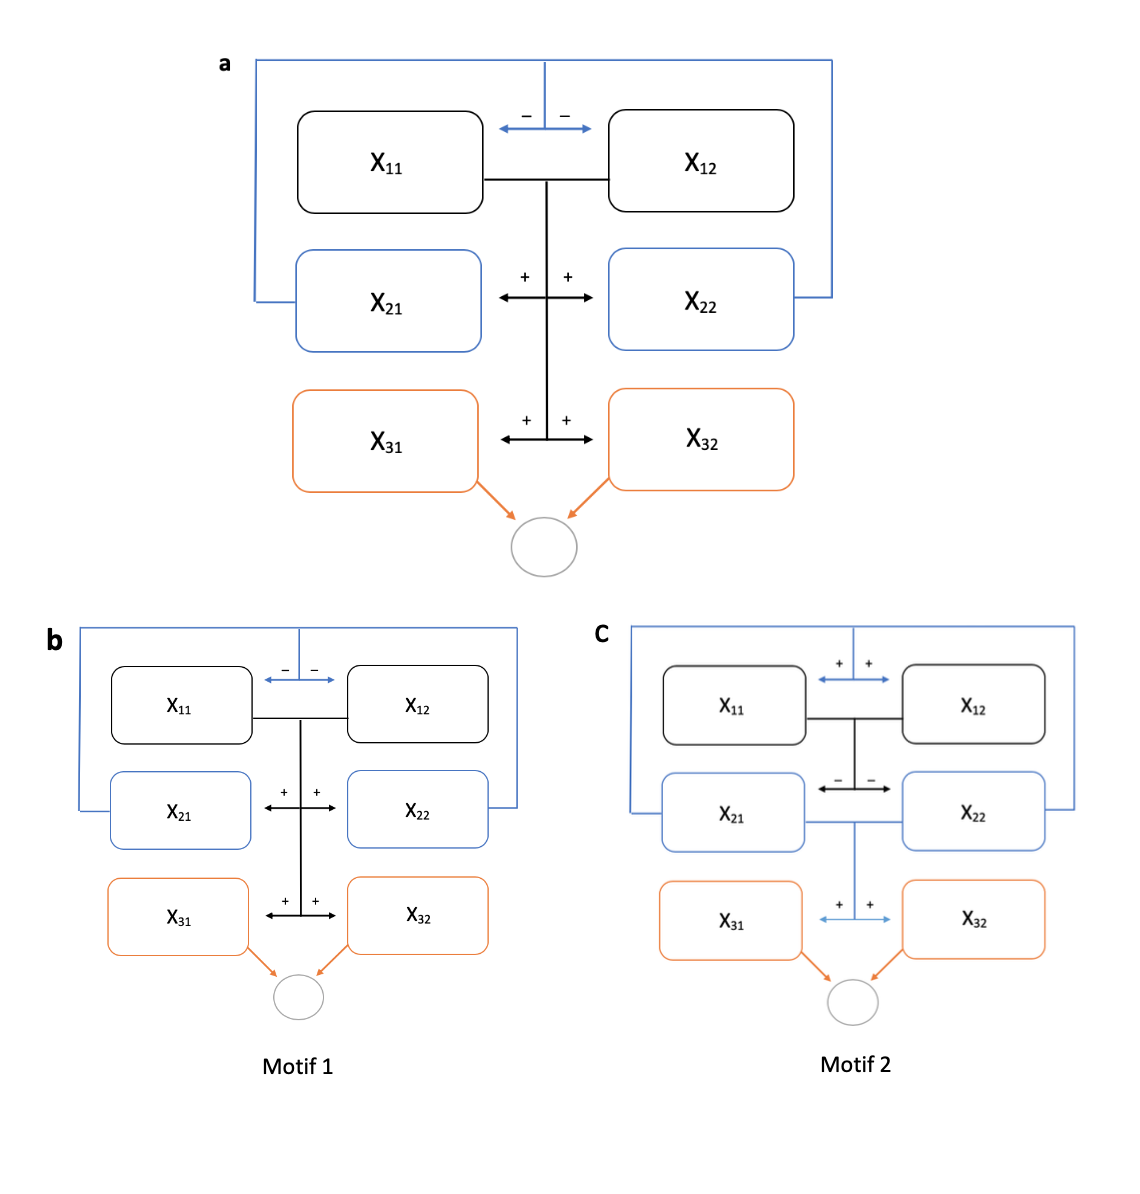
\includegraphics[scale=0.35]{../Results/Model_diagram.jpg}
    \end{center}
    \caption{Diagram showing the genetic model and two variants used to represent the migrant population. (a) Interlocus model of the population in focus. Lines labelled with mathematical symbols showing the interactions between genes. Gene $X_1$ interacts with both gene $X_2$ and $X_3$, positively regulating both of them. To limit site values below infinity, gene $X_2$ is reponsible for negatively autoregulating $X_1$. There is an output for each gene where $j = {1,2}$ and $y_j = x_{j1} + x_{j2}$. Gene $X_3$ contains the trait values for each individual, which is the output. Circle represents phenotype which is determined from trait values using a Cauchy Distribution. (b) and (c) represent models for the migrant population. (b) is the same pathway and regulation as (a) however (c) is switched where gene $X_1$ negatively autoregulates $X_2$, and gene $X_2$ positively regulates $X_1$ and $X_3$. Again, output of gene $X_3$ are the trait values used to derive fitness.}
    \label{fig:Starting parameters}
\end{wrapfigure}
Where $y_j$ is the total protein concentration at each gene. There are four sites which represent the different factors affecting protein production. These are \textit{\textalpha}, \textit{\textgamma}, \textit{\texttheta} and $P$. \textit{\textalpha} is the protein production rate while \textit{\textgamma} is the degradation rate \cite{omholt2000gene}. For both sets of populations, a single gene, $X_3$ determines the trait value for individuals and quantifiably differentiates the populations in terms of morphology \cite{orr2001genetics}. For the population in focus, gene $X_1$ positively regulates gene $X_2$ and gene $X_3$, and gene $X_1$ is negatively regulated by gene $X_2$. This is to regulate trait value and prevent the value from exceeding to infinity. As gene $X_2$ increases in expression, it decreases $X_1$ expression, negatively autoregulating the system and limiting its value. Let $j = {1,2,3}$ and $i = {1,2}$, from the separate researches of \textit{Omholt (2000)}, and \textit{Gjuvsland (2007)}, $R_{j}$ is a regulatory Hill Function representing a Michaelis-Menten mechanism, where $S(y_j,\theta,P) = \frac{y_j^P}{y_j^P+\theta^P}$. The Hill Function explains the relationship between regulator and producer, where \texttheta is the amount of regulator needed for 50\% production rate and P affects the steepness of the curve \cite{gjuvsland2007statistical,omholt2000gene}. Should the network be negatively regulated, it leads to the following equation:
\begin{equation*}
    R_{j}(y) = 1 - S(y, \theta_j , P_j), j = {1, 2} \label{eq:Negative autoregulation function} \tag{2}
\end{equation*}
And if positively regulated:
\begin{equation*}
	R_{j}(y) = S(y, \theta_j, P_j), j = {1, 2} \label{eq:Positive autoregulation function} \tag{3}
\end{equation*}
Again, letting $j = {1,2,3}$, as gene $X_1$ positively autoregulates gene $X_2$ and gene $X_3$, and gene $X_2$ negatively autoregulates gene $X_1$, this results in the following equations:
\begin{equation*}
    R_{1j}(y_2) = 1 – S(y_2, \theta_{2j}, P_{2j}) \label{eq:X1 negative autoregulation function} \tag{4.1},
\end{equation*}
\begin{equation*}
    R_{2j}(y_1) = 1 – S(y_1, \theta_{1j}, P_{1j}) \label{eq:X2 positive autoregulation function} \tag{4.2},
\end{equation*}
\begin{equation*}
    R_{2j}(y_1) = 1 – S(y_1, \theta_{3j}, P_{3j}) \label{eq:X3 positive autoregulation function} \tag{4.3}
\end{equation*}
\textit{\textmu} is the ratio of \textalpha and \textgamma per locus. Using the equilibrium solutions, total protein concentration is calculated by the following equations:
\begin{equation*}
    y_1 = \mu_{11}(1 – S(y_2, \theta_{21}, P_{21})) + \mu_{12}(1 – S(y_{2}, \theta_{22}, P_{22})) \label{eq:y1 function} \tag{5.1}
\end{equation*}
\begin{equation*}
    y_2 = \mu_{21}(S(y_{1}, \theta_{11}, P_{11})) + \mu_{22}(S(y_{1}, \theta_{12}, P_{12})) \label{eq:y2 function} \tag{5.2}
\end{equation*}
\begin{equation*}
    y_3 = \mu_{31}(S(y_{1}, \theta_{31}, P_{31})) + \mu_{32}(S(y_{1}, \theta_{32}, P_{32})) \label{eq:y3 function} \tag{5.3}
\end{equation*}
\subsection{Migrant network}
For the first motif, the genetic network will be the same as the main population, just evolving to a different local optimum trait value of either 65 or 80. For the second motif however, the difference is that gene $X_1$ negatively regulates gene $X_2$, while gene $X_3$ and gene $X_1$ are positively regulated by gene $X_2$. The formulas used to derive $y_1$, $y_2$ and $y_3$ values for the migrant population are as follows:
\begin{equation*}
    y_1 = \mu_{11}(S(y_2, \theta_{21}, P_{21})) + \mu_{12}(S(y_2, \theta_{22}, P_{22})) \label{eq:y1 function} \tag{6.1}
\end{equation*}
\begin{equation*}
    y_2 = \mu_{21}(1 – S(y_1, \theta_{11}, P_{11})) + \mu_{22}(1 – S(y_1, \theta_{12}, P_{22})) \label{eq:y2 function} \tag{6.2}
\end{equation*}
\begin{equation*}
    y_3 = \mu_{31}(S(y_2, \theta_{31}, P_{31})) + \mu_{32}(S(y_2, \theta_{32}, P_{32})) \label{eq:y3 function} \tag{6.3}
\end{equation*}
This is to represent the concept of differentiated species but can still integrate in the other population and interbreed.
\subsection{The simulation}
A total of 44 permutations based on conditions in \textit{(see Appendix A)} of environmental distance, genetic network structure, migration rates and migration patterns were simulated for 1,200 generations each run. For the effect of genetic drift and to account for the large deviations of values, a Cauchy distribution is used to generate fitness probabilities per generation. Since the Cauchy distribution is characterized for its heavy tails. The values entered in the Cauchy distribution are the desired trait values. It is important to note that environment is kept constant. Both populations were kept constant at 500 individuals. The main population evolved to a trait value of 50 with a standard deviation 8, while the migrant population alternated between 65 and 80 with standard deviation 10. The large standard deviations characterise the varying forms of morphology that can be noticed in species. The trait values represent the environments of both populations and the local optimums they evolve to.\\
For the simulation we assume that both populations have the same size and stay constant, with migrants replacing individuals.  There is no spatial structure and all individuals have an equal chance of being replaced. Both populations undergo divergent selection, stabilising in their own environments to different specified trait values, thus differentiating the populations over time \cite{sato2006effect}. Alleles for each individual can either be homogenous, using a uniform distribution to determine starting value between 0.1 and 0.3 for both populations, or heterogenous, using a uniform to randomly generate the starting allele values, again between 0.1 and 0.3. If the population is homogenous, each individual in the population starts with the same value at each locus, otherwise have differing values if heterogenous.
Recombination is equal chance at any locus and interchanges the alleles and everything downstream. Mutation can occur at each locus by randomly deviating from the current value. The probability is the same constant for both populations where each locus has an equal chance of mutating. Mutation probability is kept constant at 0.0011 per site. A mutation in the second gene will have trans-regulatory effects as gene $y_2$ negatively autoregulates gene $y_1$, while the effect of gene $y_1$ will affect the expression values of gene $y_3$. Since all genes in the model represent regulatory and coding regions, mutations in any site can be considered to affect phenotype, for its pleiotropic effects \cite{rice2019evolution; landry2007genetic}.\\
Fitness is reproductive success, or the probability of being a parent and passing on their allele values which is determined by phenotypic value. Each individual per generation has no limit as to how many times they can be a parent, however the standard deviation of 8 and 10 in the Cauchy distribution attempts to produce varying combination of parents. Migration rates varied between 1\%, 3\% and 5\%. As migrant individuals enter the population, they randomly replace individuals in the population. With constant population size, this represents immigration and emigration. Furthermore, low migration rates were used to prevent migration population from completely replacing the original population and allowing the network to be able to adapt to the new values. Both populations have a burn-in period of 80 generations to evolve in their own environments before migration can happen. Also, migration only occurs till the 700th generation. The remaining 500 generations are to assess how the network responds to the migration. Patterns of migration were also considered, varying between each generation, every 10 generations, every 5 generations and random (between 1\% and 5\% each occurrence) after the 80th generation.
\subsection{Analysis}
Analysis was done on the recorded fitness, trait values and population arrays. At the end of each simulation, fitness is normalised by dividing fitness probabilities with the median of Cauchy distribution for the local population, with 1.0 being the highest possible fitness value. Firstly, control conditions of no migration were simulated to see how rapidly isolated networks evolve. Without migration, I expect rapid evolution of allele values, especially for the heterogenous population due to varying alleles present \cite{garcia1997genetic}. To analyse robustness, I calculate a robustness ratio. The fittest individuals before and 10 generations after migration were recorded and replicated such that there were 4 separate mutations per site. Trait values were again inputted into the Cauchy distribution to determine fitness values. The robustness ratio is then the variance in fitness after migration divided by variance in fitness before migration. Ratios were then log transformed as to linearise and make it less skewed. A negative value is thus desired for robustness and analysis of variance test is done to see if any factors significantly contribute to robustness.


\newpage

\section{Results}
% ITEX root = ../thesis.tex
\subsection{Cauchy Distribution}
\begin{wrapfigure}{r} {0.7\textwidth}
    \begin{center}
        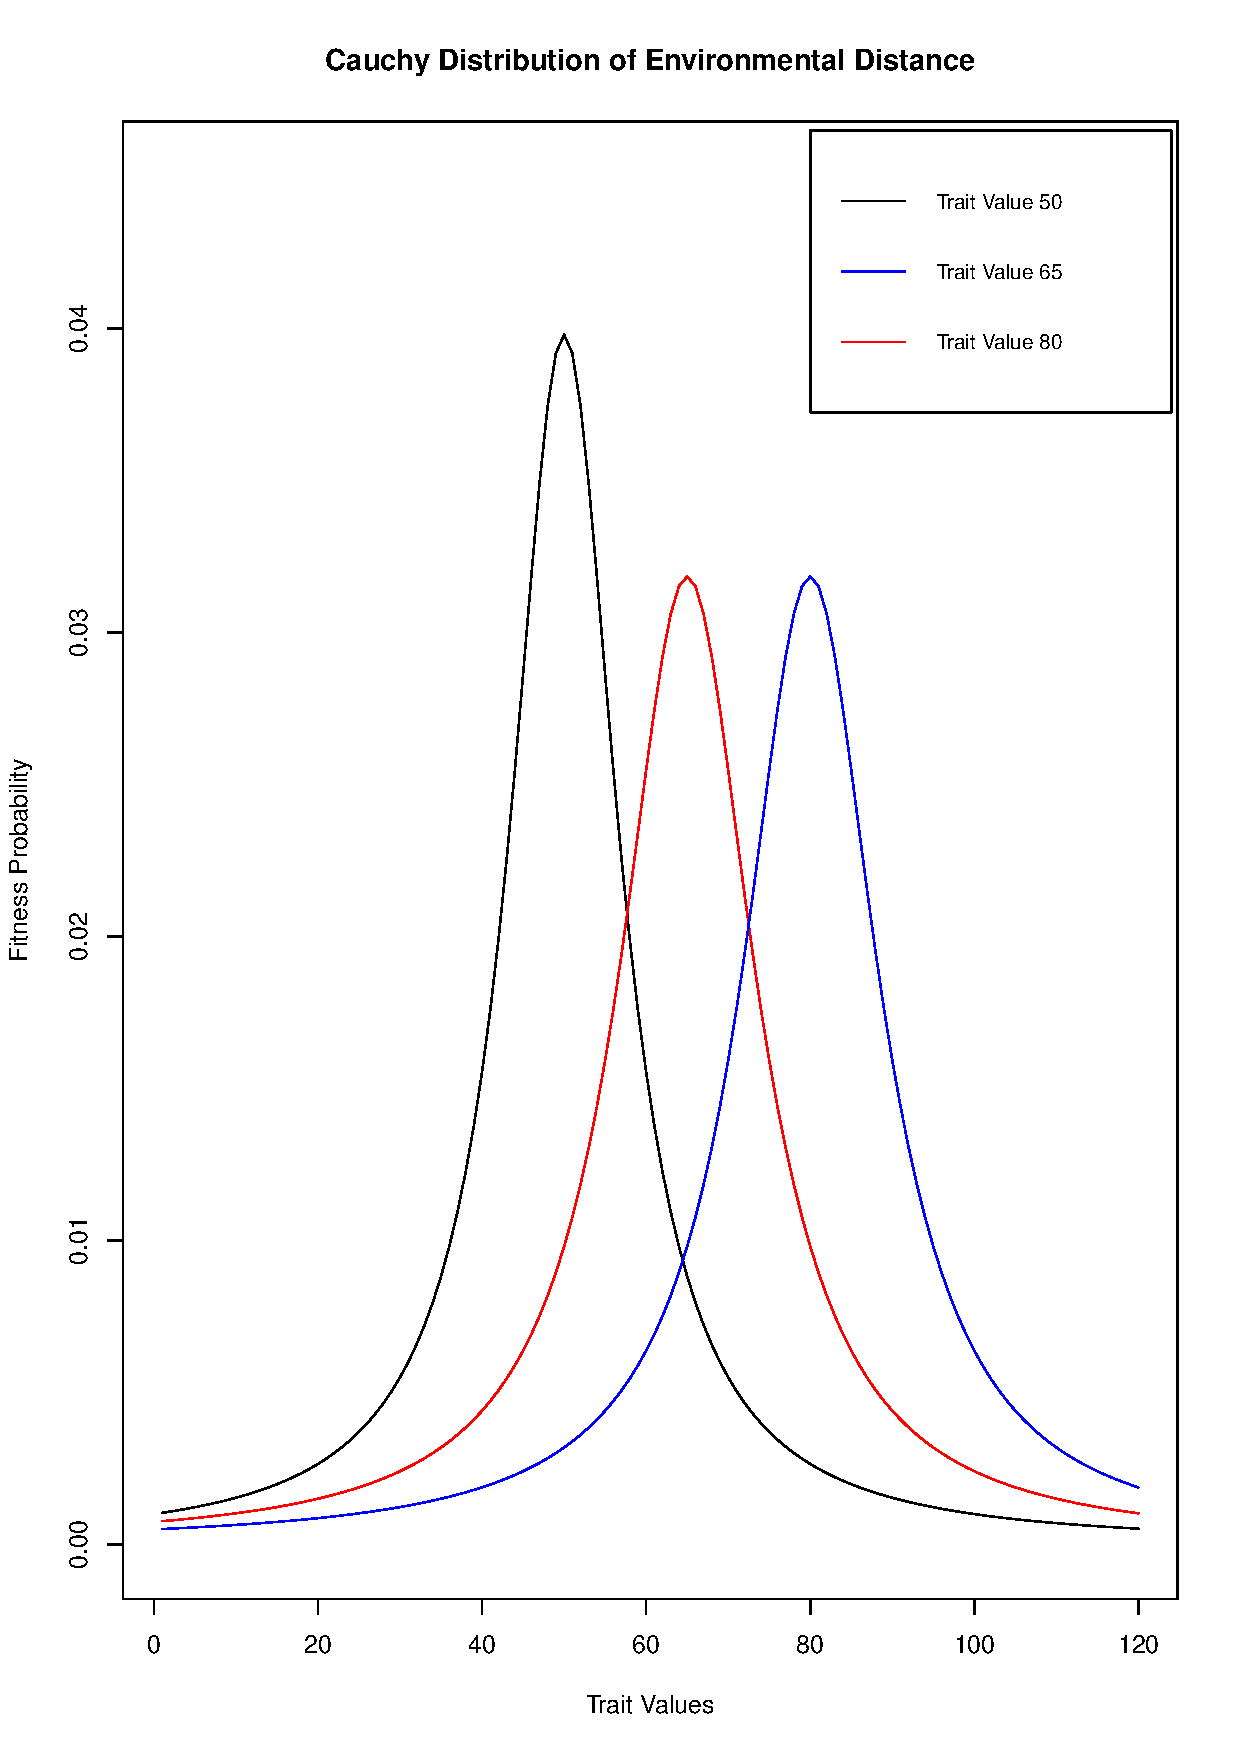
\includegraphics[scale=0.2]{../Results/Cauchy_Distribution.pdf}
    \end{center}
    \caption{Plot of the Cauchy Distribution used to derive fitness probabilities (for reproduction) and fitness values (normalising) of individuals. Distribution is also representative of the environmental distances respective populations evolved to. The main population (black) evolved to a trait value of 50, where the peak trait value has a reproductive probability of 3.98\%. Migrant populations either evolved to a trait value of 65 (blue) or 80 (red).}
    \label{fig:Cauchy Distribution}
\end{wrapfigure}

\textit{Figure 2} on the shows how the trait values are distributed along a Cauchy distribution. These desired trait values represent the environment and the distance between them is the environmental distance. The values must not be too far apart that the probability is 0, meaning that migrant genes are passed on to future generations and we see how the network develops with invading alleles. Since the Cauchy distribution is long tailed, this allowed for varying alleles to potentially persist in the population, as seen from the probability values along the y-axis.
\subsection{No Migration}
\begin{figure}[h!]
    \centering
        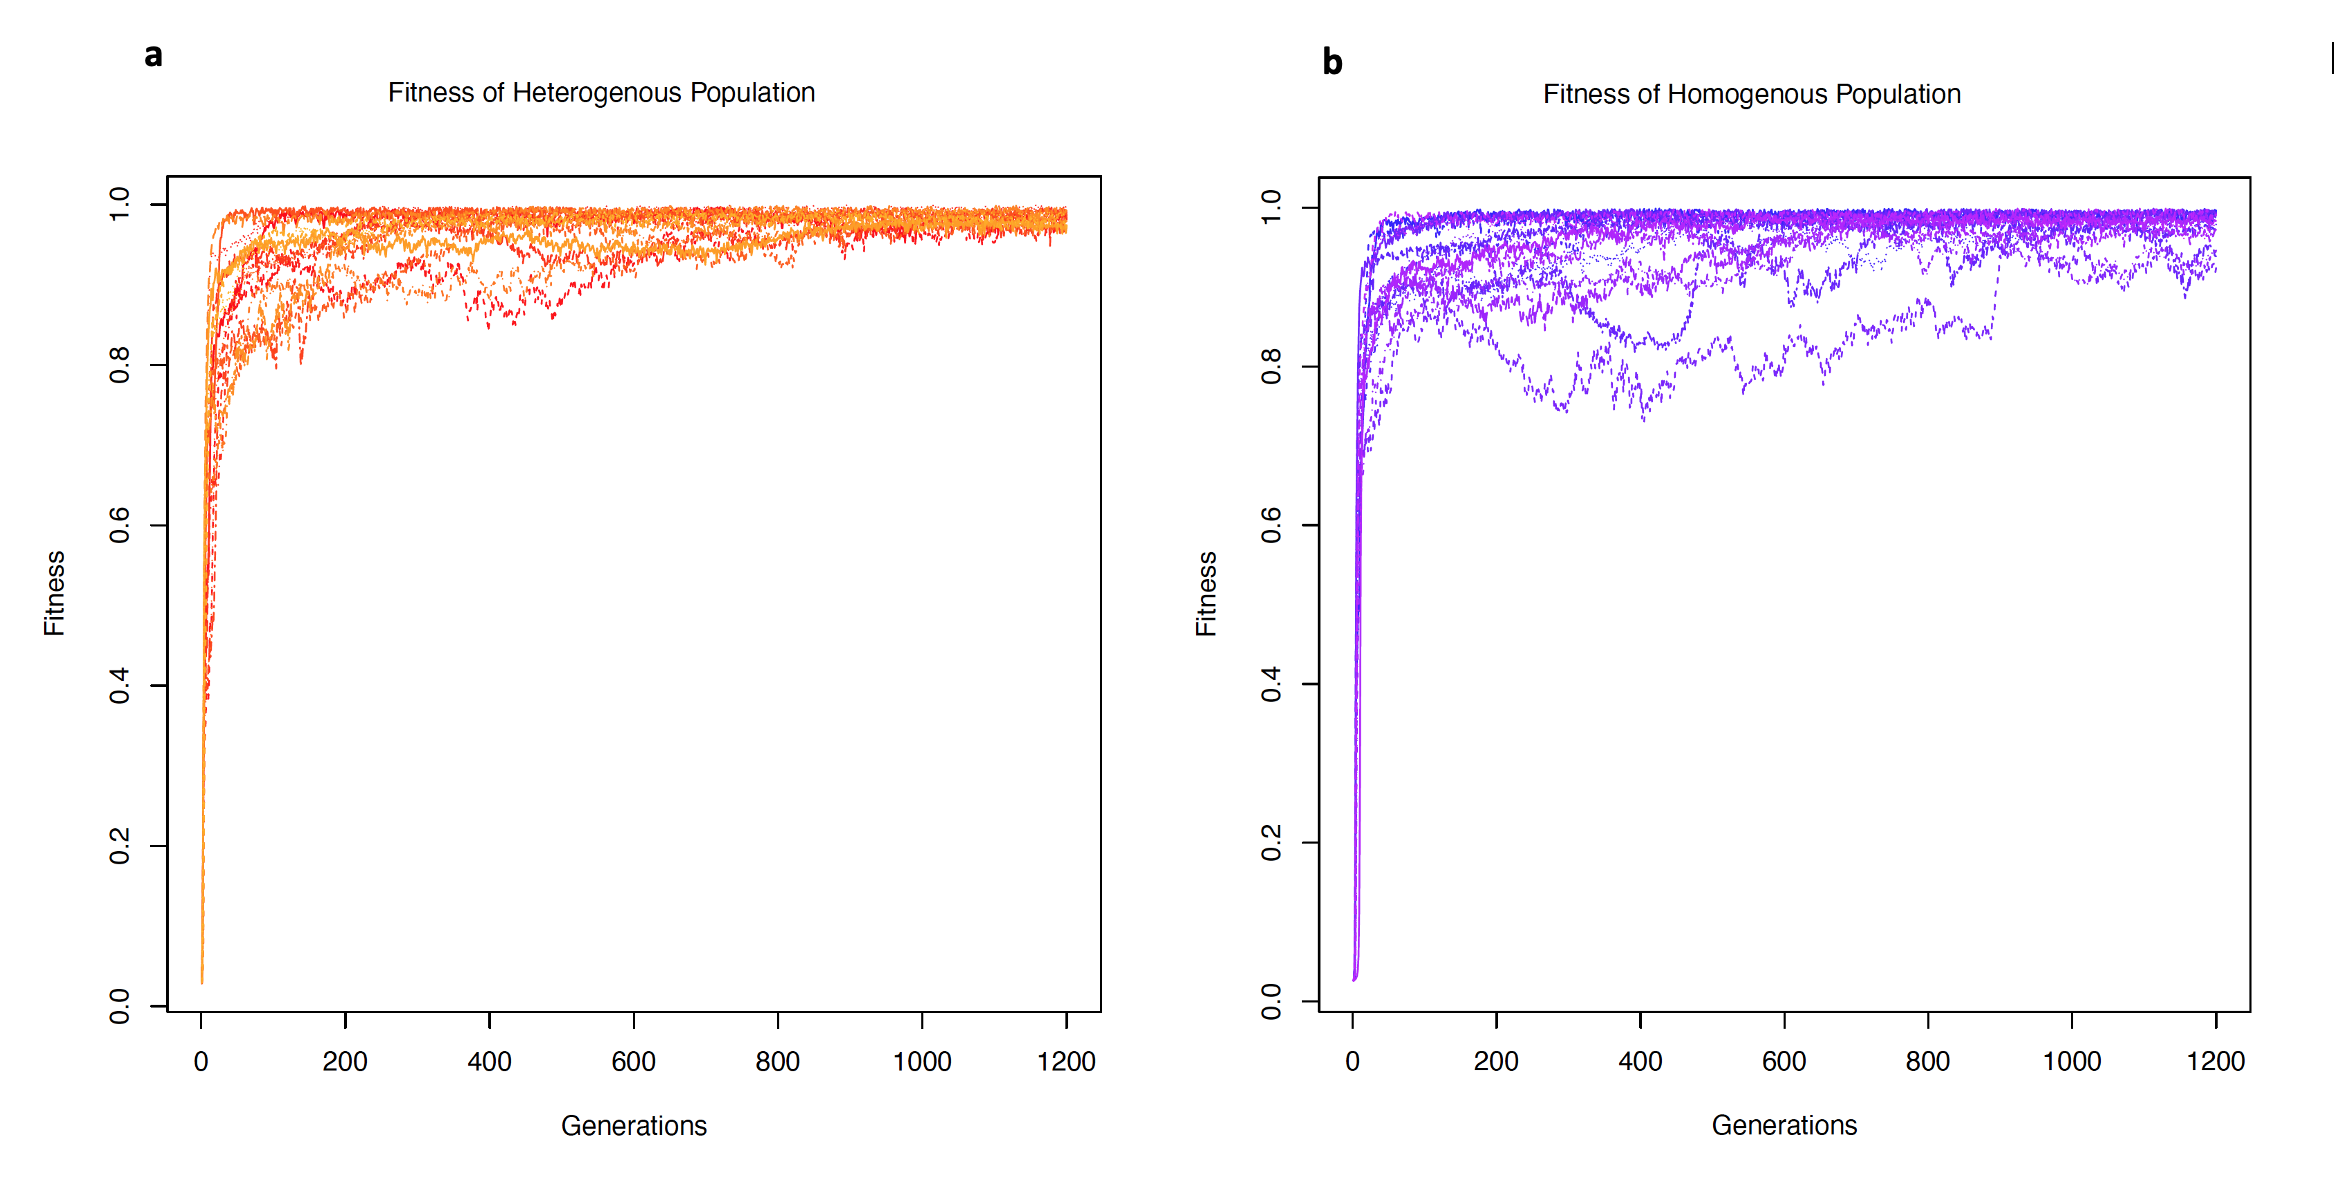
\includegraphics[width=0.9\textwidth]{../Results/no_migration.jpg}
    \caption{graphs showing the fitness evolution without migration for two different starting genetic makeups. (a) shows the evolution of a network that is homogenous network, where all starting allele values range between 0.10 and 0.30. (b) shows how a heterogenous network evolves where starting values for each allele are generated using a uniform distribution between 0.1 and 0.3. For the heterogenous populations, they had a mean fitness of 0.961, standard deviation of 0.03 while the homogenous populations had an average fitness value of 0.955 with a standard deviation of 0.05.}
    \label{fig:No Migration}
\end{figure}
When there is no migration happening, the genetic network evolves rapidly to the desired trait value. In a very short time period, it reaches an average fitness of 0.919. This can be seen from \textit{figure 3} to the right. After normalising the fitness, once the trait values of individuals however around 50, the fitness staggered close to maximum fitness, sometimes going below. When plotting the average fitness values of homogenous and heterogenous, they both show rapid evolution and have very similar patterns. Furthermore, this is seen in \textit{figure 6} which is a boxplot showing the distribution of the number of generations needed to reach the average fitness for with and without migration. It quickly rises to around 0.90 and slowly plateaus, stabilising close to 1.00, highest possible fitness. No migration overall resulted in a high average fitness, with a value of 0.958 and standard deviation of 0.04.
\subsection{Migration}
\begin{figure}[h!]
    \centering
        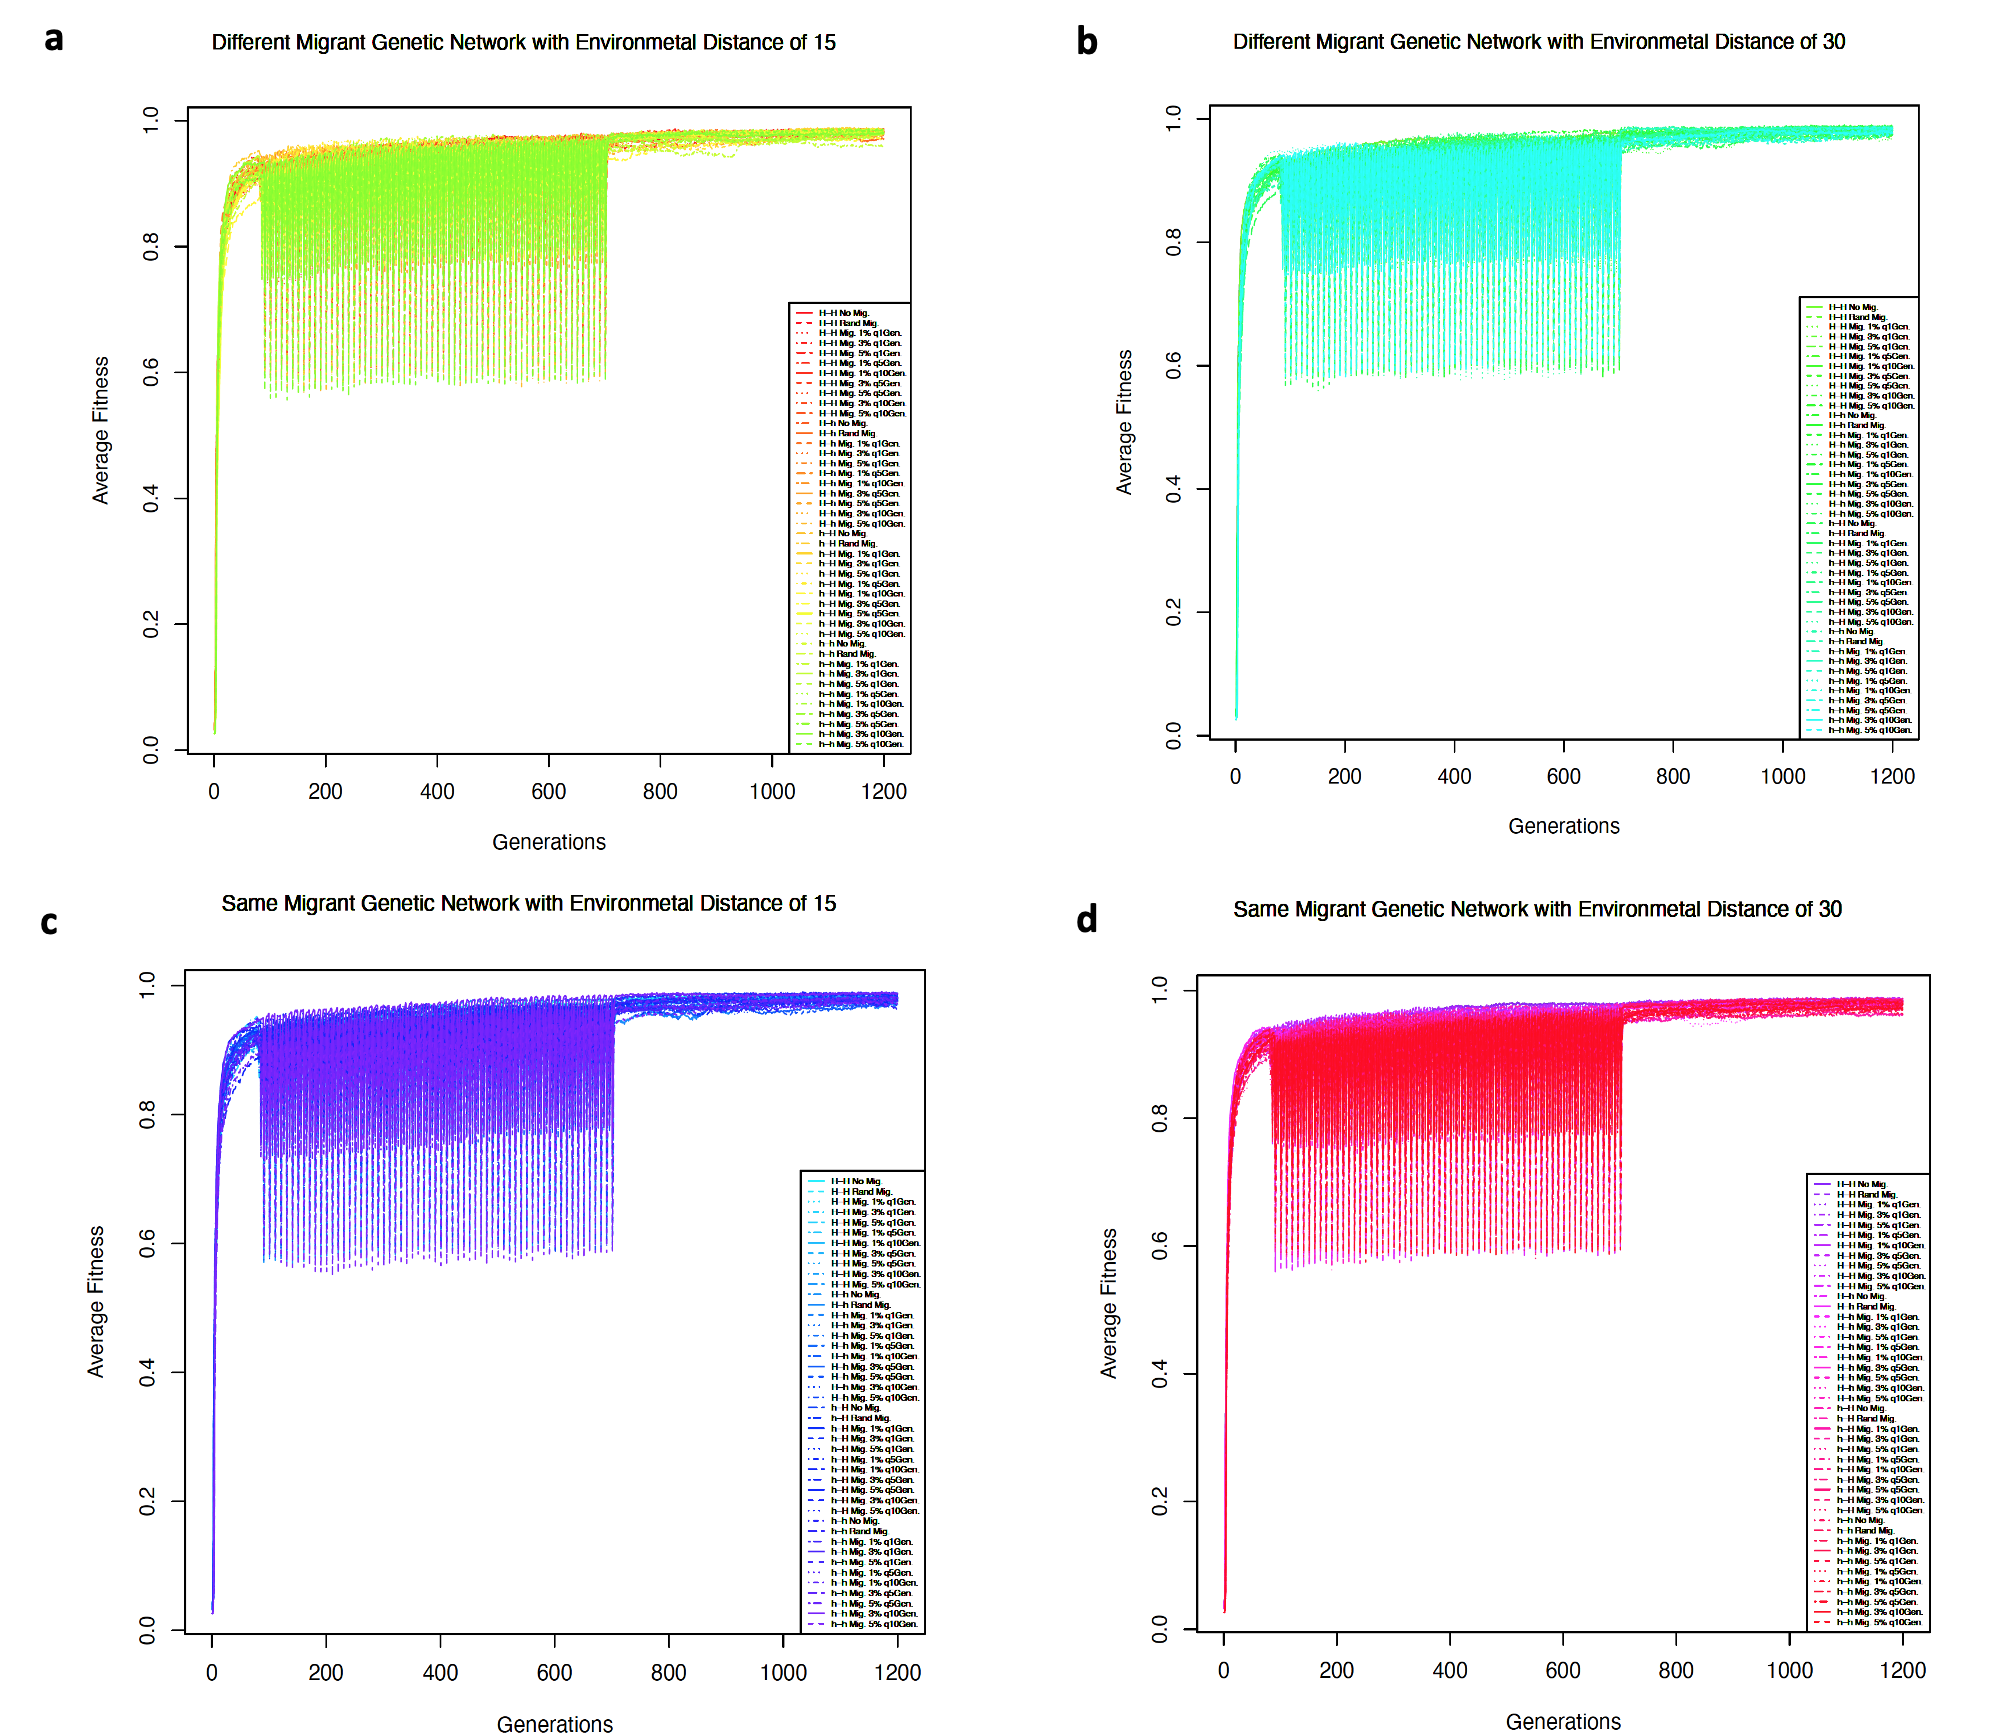
\includegraphics[width=0.9\textwidth]{../Results/migration.jpg}
    \caption{Plots showing the effect of migration on fitness over time. Migration occurs between generations 80 and 700, where the network gets 500 generations afterwards to try and recover. The graphs show how migration caused fluctuations in fitness values (a) shows the effect of migrant network with different regulations from the main population, evolving to a trait value of 65 (Environmental Distance of 15). It is a variation where gene $y_1$ negatively regulates gene $y_1$, and gene $y_2$ positively regulates the other genes, including gene $y_3$ which is the trait values. Mean fitness was 0.917, with a standard deviation of 0.069. (b) is a migrant network same as in graph (a) where the regulations are different, instead evolving to 80 (Environmental Distance of 30). Mean fitness value was 0.070, standard deviation of 0.070. (c) shows the effect of a migrant population but with the same regulations as in the main population. Therefore, gene $y_2$ is negatively regulated by gene $y_1$, and gene $y_1$ positively regulates the other genes. Similar to graph (a) it is evolving to a trait value of 65. Mean fitness of 0.917 and standard deviation of 0.071. (d) same regulation as the migrant network in graph (c) however evolves to a trait value of 80. Mean fitness of 0.916 and standard deviation of 0.071.}
    \label{fig:With Migration}
\end{figure}
\\
\begin{figure}[h]
    \centering
        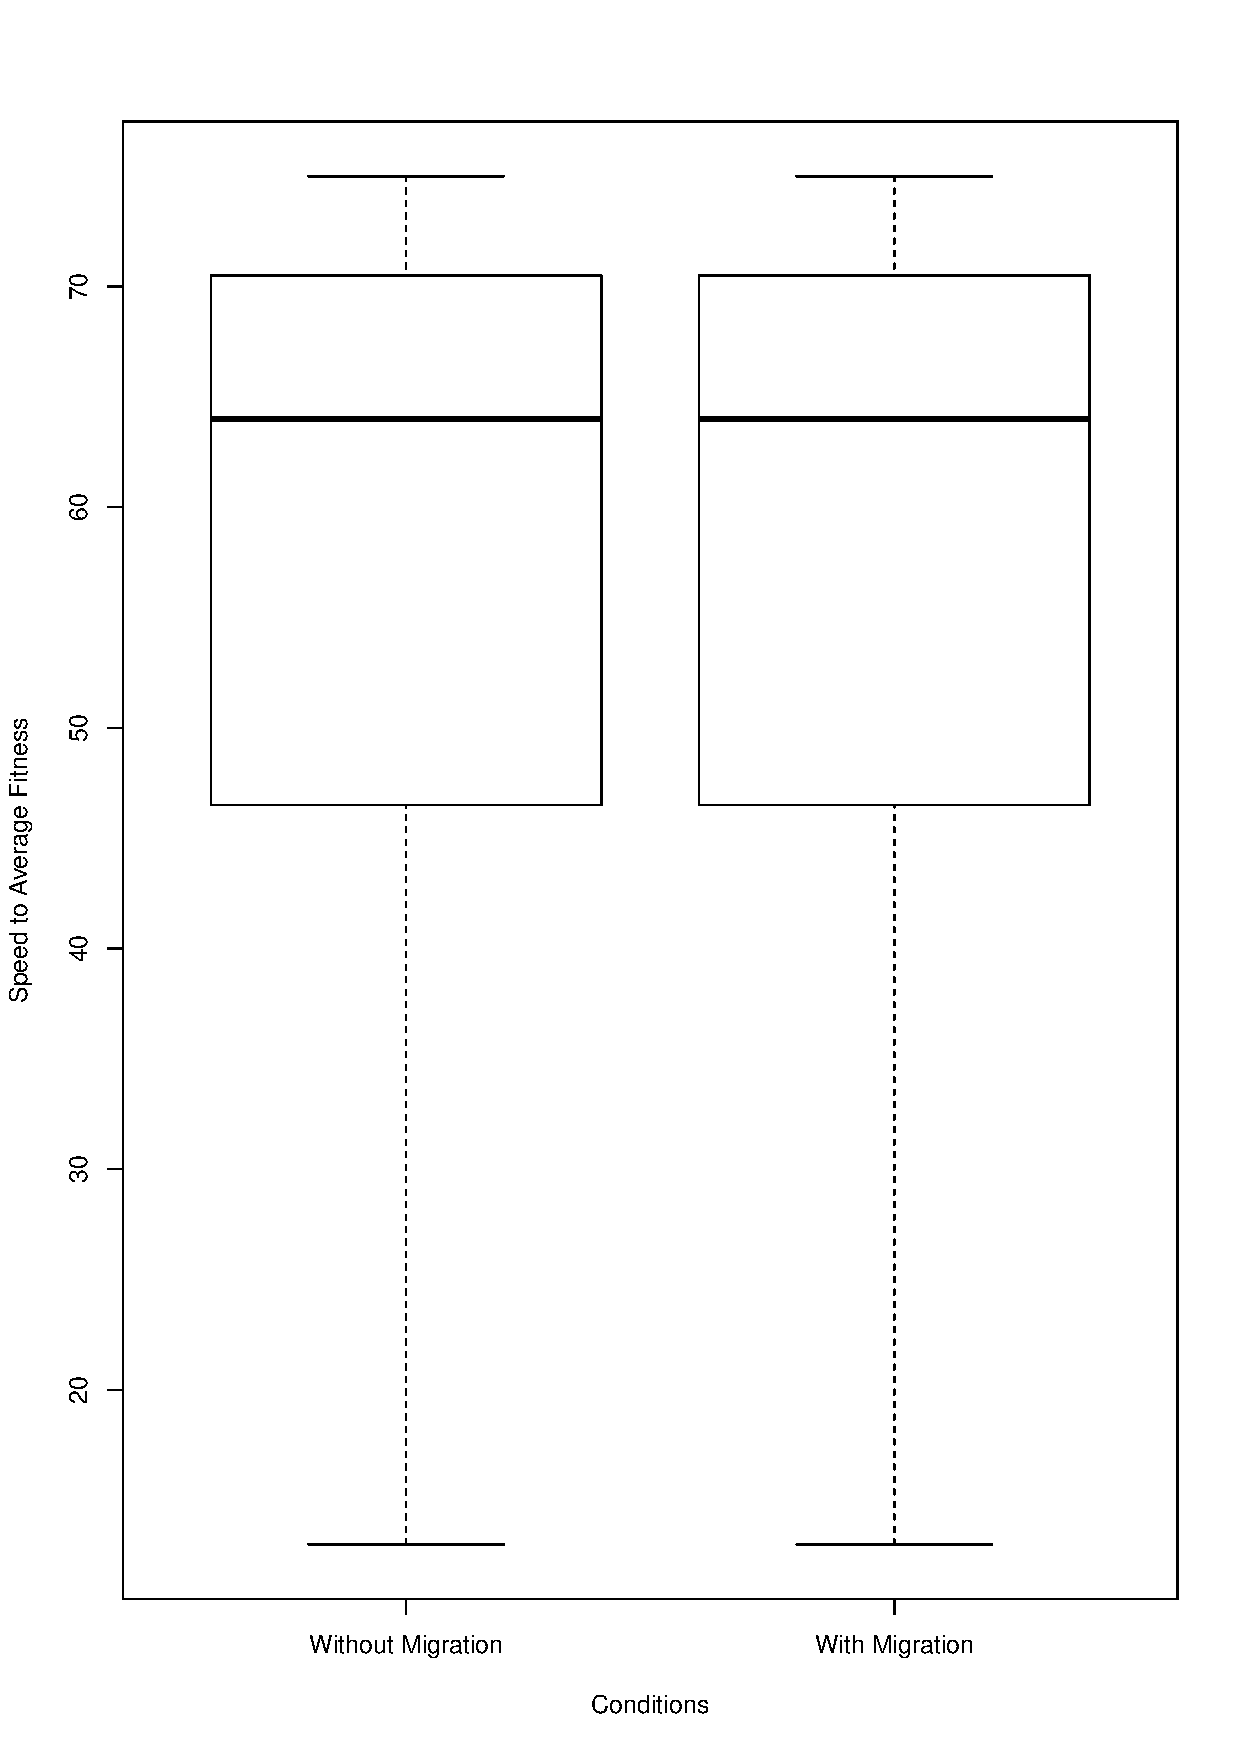
\includegraphics[width=0.8\textwidth]{../Results/boxplot_migration.pdf}
    \caption{Boxplot showing the number of generations taken to reach the average fitness of both conditions, with and without migration. When there is no migration, it takes an average of 57.4 generations (standard deviation of 15.58) to reach an average fitness value of 0.919 (standard deviation of 0.05). When migration is present, it takes an average of 57.4 generations (standard deviation of 15.55) to reach an average fitness value of 0.918 (standard deviation of 0.05).}
    \label{fig:Speed to average fit}
\end{figure}
With migration, the genetic network evolved the same as without migration. It took an average of 57.4 generations (standard deviation of 15.55) to reach an average fitness value of 0.918 (standard deviation of 0.05). The genetic network showed to evolve rapidly without migration and as well with migration as it did not affect the networks early evolution since migration did not begin till the 80th generation. The mean speeds were the same but differed was a slightly in terms of variance. This is shown in the boxplot in \textit{figure 6} to the right. The expectation was that migration would hinder the structures ability to evolve and it would take more generations to reach the average fitness. The effect of migration was seen in the variance of fitness from the plots in \textit{figure 5}. When there was migration, the fitnesses was fluctuating and going below 0.50. This was to be expected as maladaptive foreign

alleles cause the trait value and fitness to deviate from the local optimum. The variation between the different genetic structures and environmental distances was very low as conditions generated similar fitnesses and variance during periods of migration. In the periods of migration (80th generation – 700th generation), the average fitness 0.916 and a standard deviation 0.071.



\section{Discussion}
% ITEX root = ../Campos_Matthew_CMEE_2020.tex
\subsection{No Migration}
Previous studies showed how a reproductively isolated population would evolve rapidly \cite{garcia1997genetic}. Without gene flow, populations did evolve rapidly to their environment due to a balance between selection and drift \cite{garcia1997genetic,tigano2016genomics,barber1999patterns}. Especially for a heterogenous genetic network, which would evolve a lot quicker which was the case. Compared to a population that started as homogenous, heterozygous individuals had variation in allele values at the start allowing for better combinations of values for selection to act on. This allowed such values to propagate and spread in the population. Swift rise (within 100 generations) can be attributed to the fitness distribution and the non-limitations in reproduction of the simulation. Following the fitness distribution, the most fit individuals per generation were likely to have been selected for reproduction many times allowing their combination of alleles to be passed on at a high frequency. Thus, the slopes of the heterogenous plots in \textit{figure 3} are steep, suggesting selection was strongly acting on the population. Deviations seen are likely due to mutation and recombination events that removed favourable allele values and combinations.\\
In the homogenous case, the instances where fitness rose close to 1 is likely due to chance beneficial mutations and recombination to create better combination of allele values, and epistasis which drive the adaptiveness \cite{tigano2016genomics}. A beneficial mutation in $gene_1$ for example can have positively consequences for the values in $gene_2$ and $gene_3$. With selection and non-limiting reproduction acting on the system, it allows for such values quickly spread in short time, raising the fitness of the population. Additionally, \textit{figure 2} shows the magnitude in difference of deviating towards from the median of the distribution. For the desired trait value of 50 with a standard deviation of 8, the maximum probability an individual has of being chosen is 3.98\%. Although this is a small value, an individual that is 10 trait values away will have a probability of 1.55\%, a three-fold difference between them. So, selection and limitless parental contribution allows even a small number of fitter individuals to be parents many times and pass on their values.
\subsection{Migration and Robustness}
To begin with genetic regulatory pathway of a population is seen to effect recovery time. Boxplot in \textit{figure 5} shows that recovery time for a migrant population with a different regulatory network, one that evolves to a trait value of 65, and same regulatory system evolving to trait value 80 are quickly diminished from the population. However, a different migratory network that evolves to 80 or the same migratory network evolving to 65 persists in the population longer. Other than beneficial mutation or recombination events, there could be a possibility that gene flow helped to improve fitness. That patterns caused by evolutionary forces could be context-dependent. For a homogenous population that evolves slowly in, gene flow could lead to variant alleles closer to the peak of the distribution, hence a greater number of rising peaks in \textit{figure 4b and 4c}. Further runs and tests must be conducted to statistically observe if gene flow has a beneficial effect depending on environmental distance and genetic makeup.\\
For heterogenous populations, \textit{figure 4} shows how gene flow has an expected negative effect on fitness. It leads to large deviations in the fitness. Poorly adaptive traits to the environment would delay the system ability to evolve to local optimum as the values deviate far from it \cite{garcia1997genetic}. This was to be expected as periods where the foreign alleles far from the peak of the distribution. trait value and fitness to deviate from the local optimum.\\
Analysis of variance test revealed statistical significance of migration pattern on the log ratio of robustness. Although post-hoc Tukey test revealed no significance within the combinations of migration pattern, this is likely due to small sample sizes. Further testing will likely reveal significant patterns between migration rate and canalisation of a network. There was still great insight on how the genetic network was able to overcome disruptions caused by gene flow and prevent homogenizing the populations and resisting perturbations. While gene flow caused large deviations in the fitness (as seen in \textit{figure 4}), selection counteracts gene flow and maintains the adaptiveness of the network \cite{feder2012genomics,burt1995evolution}. Moreover, I could investigate the patterns at which migration, selection and drift affect population growth, analysing effect of dominance on robustness \cite{rice2009evolution,otto1999balanced}. When migrant alleles enter the population, recombination gives them the opportunity to persist \cite{feder2012genomics}. Not just migrant allele values, but also complementary combination of migrant alleles that could allow it to persist \cite{feder2012genomics}. Yet despite the presence of migrant alleles, divergent selection heavily favours local alleles in particular and is quick to remove them \cite{tigano2016genomics}. Selection favouring locally fit individuals with better combination of alleles. \textit{Feder (2012)} study highlighted a friction that exists between divergent selection, and gene flow and recombination. Results in this study show how when selection force is greater, it acts to swiftly remove migrant alleles in the population.\\
\subsection{Shortcomings and Future Work}
Due to time constraints and difficult circumstances, major assumptions were made in the model and simulation. For example, the fitness distribution in \textit{figure 2} shows how variation was quickly eliminated from the model due to the narrow shape of centre of the distribution, allowing for selection to act strongly on the network. Few trials as well of the different conditions and design of the simulation prevented significant results from appearing. Realistically, the model did not take into account spatial or temporal aspects. Species are distributed along a habitat and the environment itself can change due to perturbations i.e. vicariant events \cite{garcia1997genetic}. With more time, I would have designed a more realistic model, taking into account dispersal habits, species distribution, environment perturbations, and migration limits. Species dispersal along with varying environmental conditions would have created a more complex system and delayed the quick homogenization of the network to allow for investigation of gene flow effects on fitness \cite{garcia1997genetic,barber1999patterns,sato2006effect}. This also would better maintain the variation in the population to better analyse the impacts. This would prevent the population being completely replaced in the current model even with higher migration rates. With regards to environmental spatial dynamics, I would have made it so that different areas would have different local optimums.\\
The current simulation assumed that there is no limit to parental contribution. Since there was no limit, the fitter individuals quickly pass on their trait values in the simulation. This rapidly canalised the system and decreased the variation in the environment. To improve this, I would limit parental contribution i.e. individuals reproducing can only be parents to five next generation individuals. This would prevent the system from stabilising so rapidly and allowing for more diverse alleles to continue to propagate in the population. There were no ecological barrier restricting migration and individuals were always replaced by migrants. Random environmental perturbations that would alter local optimums would further delay network evolution allowing for longer periods of variance. Thus, the effects of selection would not so quickly evolve the system and can better investigate how network responds to disturbances. This would create more varying network structures and allow further investigation into network development with varying motifs.\\
Overall, further runs must be conducted to see effects of migration pattern on robustness. Although the post-hoc Tukey test showed no significance, it likely due to small sample size of runs per starting condition \textit{(see Appendix A)}. In addition, another aspect to research is the possible benefits of gene flow on an evolving network. More runs can give statistical insight as to whether this is the case, by tracking lineages and allele values. Moreover, I can also consider dominance and investigate how the migration, selection and drift affect population growth, analysing effect of dominance on robustness \cite{rice2009evolution,otto1999balanced}. Lastly, it would also be interesting to investigate the opposite case as to how migration patterns are influenced by these evolutionary forces \cite{w2004dispersal}.



\section{Concluding remarks and looking forward}
% ITEX root = ../Campos_Matthew_CMEE_2020.tex
In just a few centuries, anthropogenic changes largely due to societal development has disrupted many habitats and altered the evolutionary path of many species, all of which is likely to have long-term ecological consequences. This study aimed to investigate the scenario where gene flow allows related species, that could have originally been reproductively isolated, to interbreed, and the long-term impacts on species morphology and development. This can give insight into possible patterns that could emerge with future novel interactions between species to understand how development of both phenotype and genotype are altered. Although results did reveal an effect of migratory patterns on the evolution of a species network, further studies must be conducted to truly observe the interactions of environmental forces and the interplay between molecular genetic mechanisms and macro evolutionary processes. Improvement to the current simulation design and repeated trials can contribute to such studies.



\newpage

\section{Data Code and Availability}
All code can be found in the GitHub Repository:\\
{https://github.com/matthewcampos/CMEECourseWork.git}

\newpage

\bibliographystyle{agsm}
\bibliography{references}

\newpage

\begin{appendices}
\section{Permuations of Conditions}
\textbf{Description:} The different combinations of conditions used for data sorting and simulations. Data folders are permutations of Genetic structure and Environmental distance i.e. Same and 30 (Main population 50 and Migrant population 80). Within each folder are 44 combinations of starting genetic makeup of populations, migration rate and migration pattern for the simulations. For example, within Same and 30 is: homogenous - heterogenous, 3\%, every generation.
\begin{table}[h]
\centering
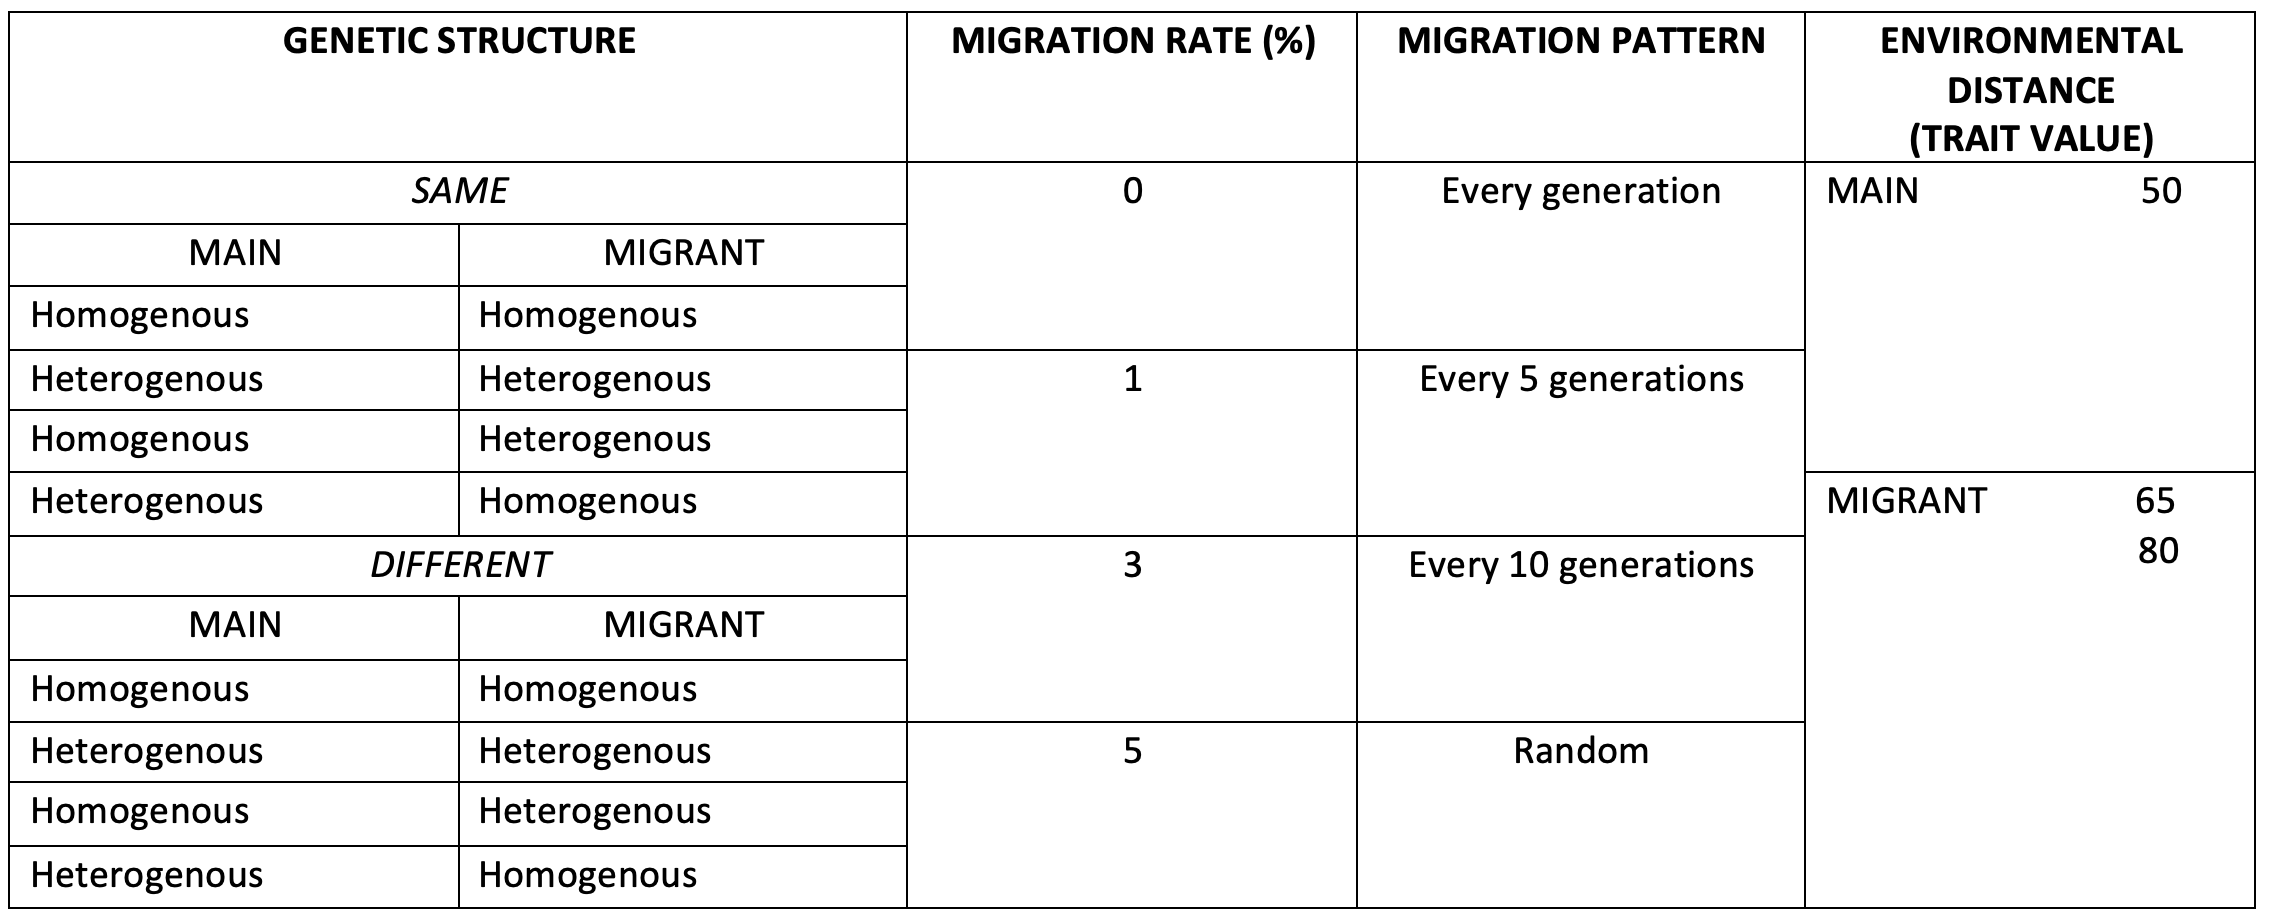
\includegraphics[scale=0.40]{../Results/AppendixI_conditions.jpg}
\end{table}

\newpage

\section{Computer Program Workflow}
\textbf{Description:} Workflow of R script of simulation program and the logic behind the design of the simulation.
\begin{figure}[h]
\centering
    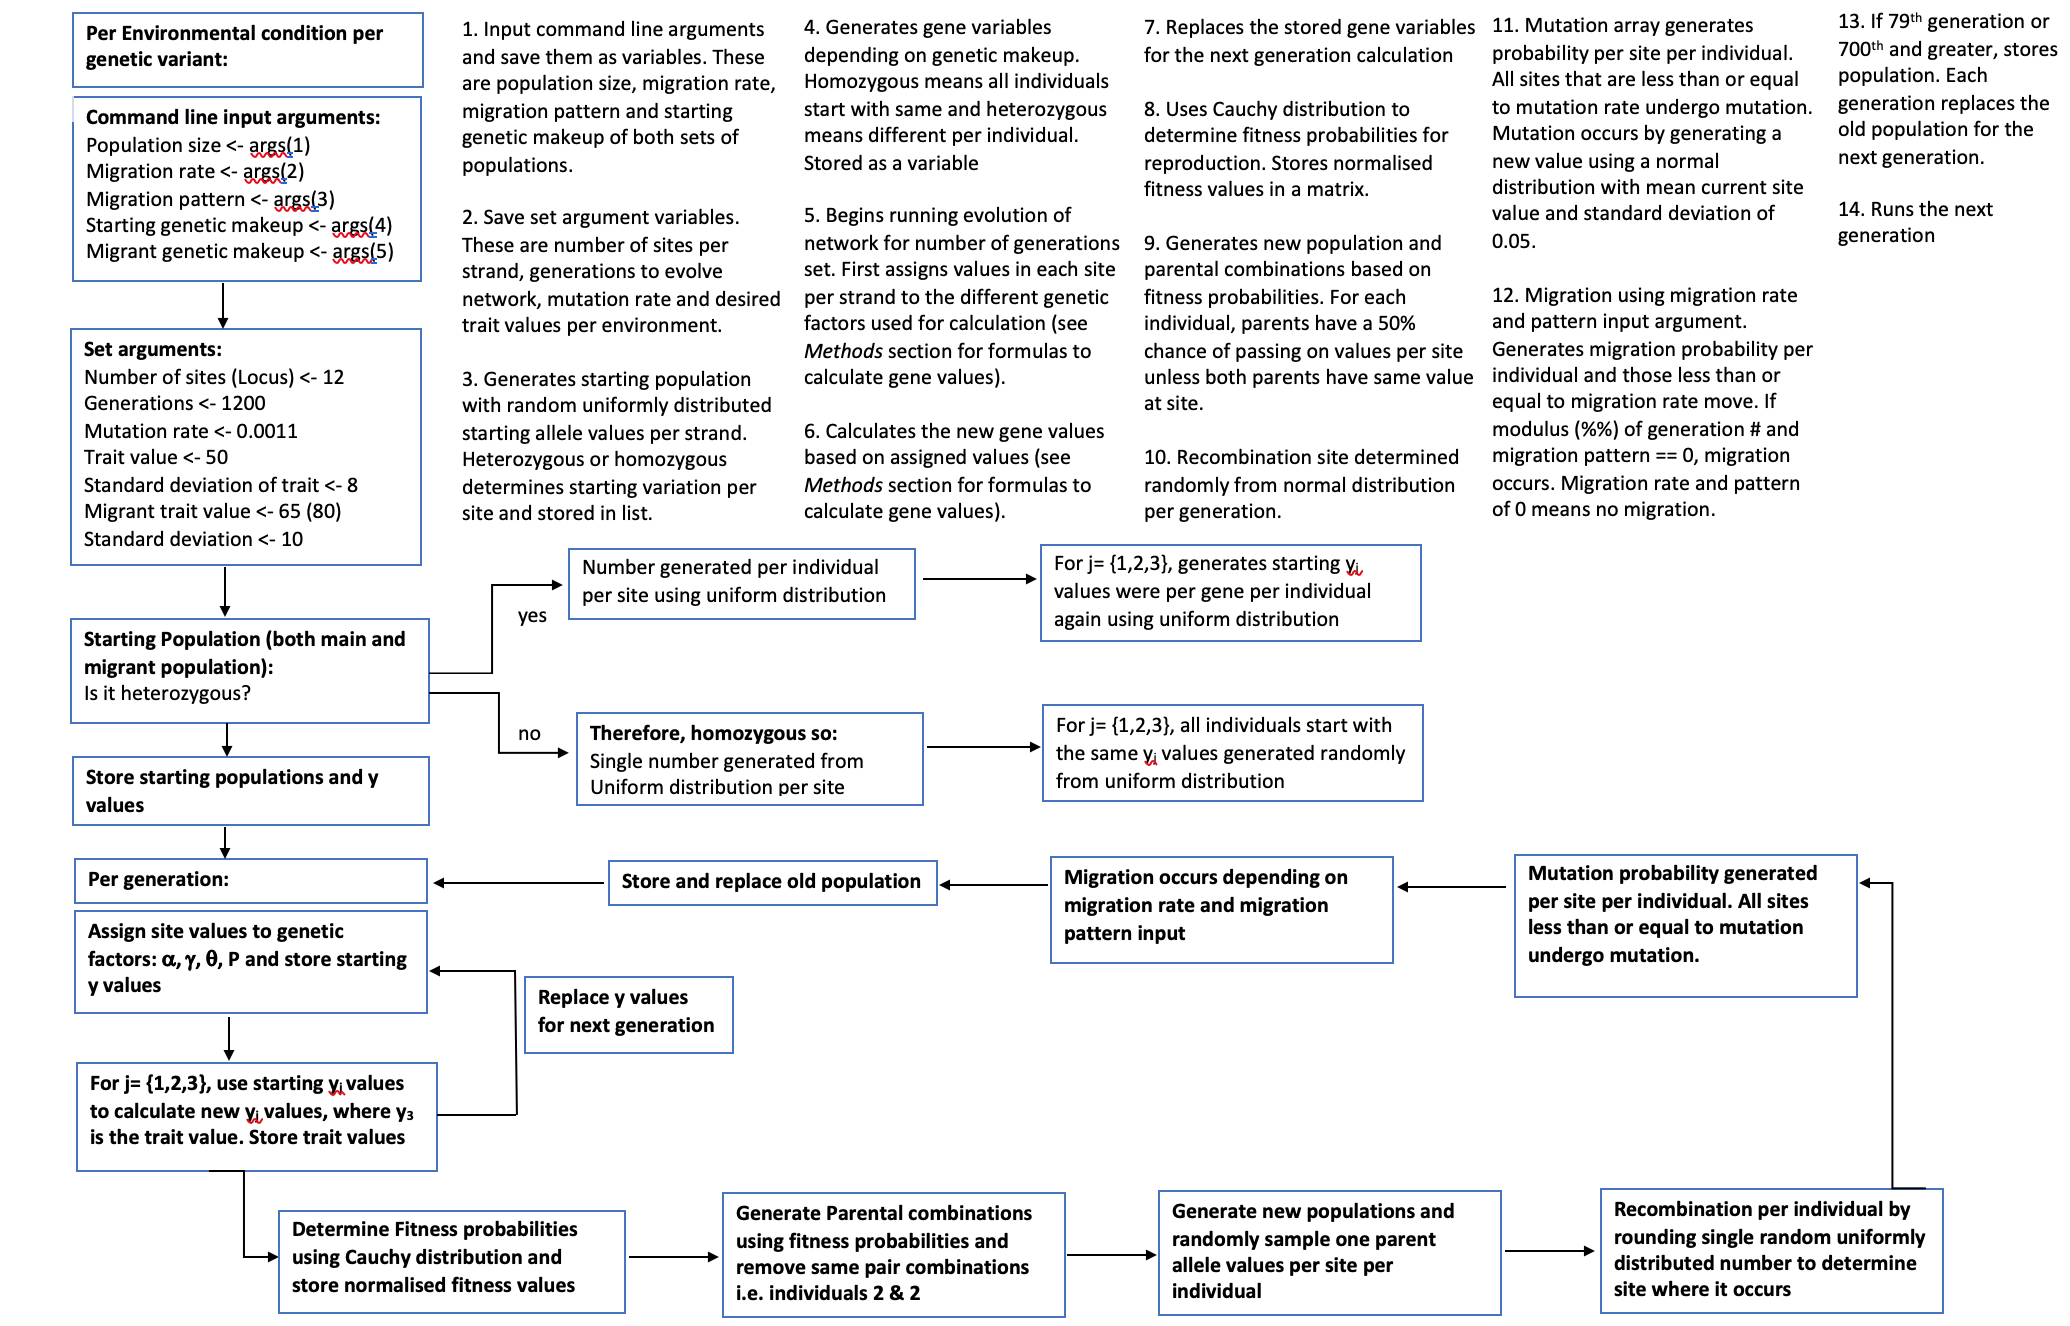
\includegraphics[width=0.9\textwidth]{../Results/workflow.jpg}
\end{figure}

\newpage

\section{Tests for One-way Analysis of Variance on Regression of the log Robustness Ratio and Migration Pattern}
\textbf{Description:} Multiple regression was conducted to see if any of the independent variables (and interactions among them) had a statistically significant effect on the log Robustness ratio. Graph (a) is a normal Q-Q plot to check if the distribution of the data was normal, with no large outliers. Distribution shows that it is a normal around the centre of the distribution however deviates a little at the ends, suggesting it is fat-tailed. This is to be expected with migrant allele values that are evolving far from the trait value. (b) is a Bartlett test conducted to see if there is homogeneity in the variances. A p-value of 0.32 so variances are equal. After conducting analysis of variance test of log Robustness ratio and Migration pattern, (c) is the post hoc Tukey test which shows no statistical significance of any particular migration pattern and the log Robust ratio.
\begin{figure}[h]
\centering
    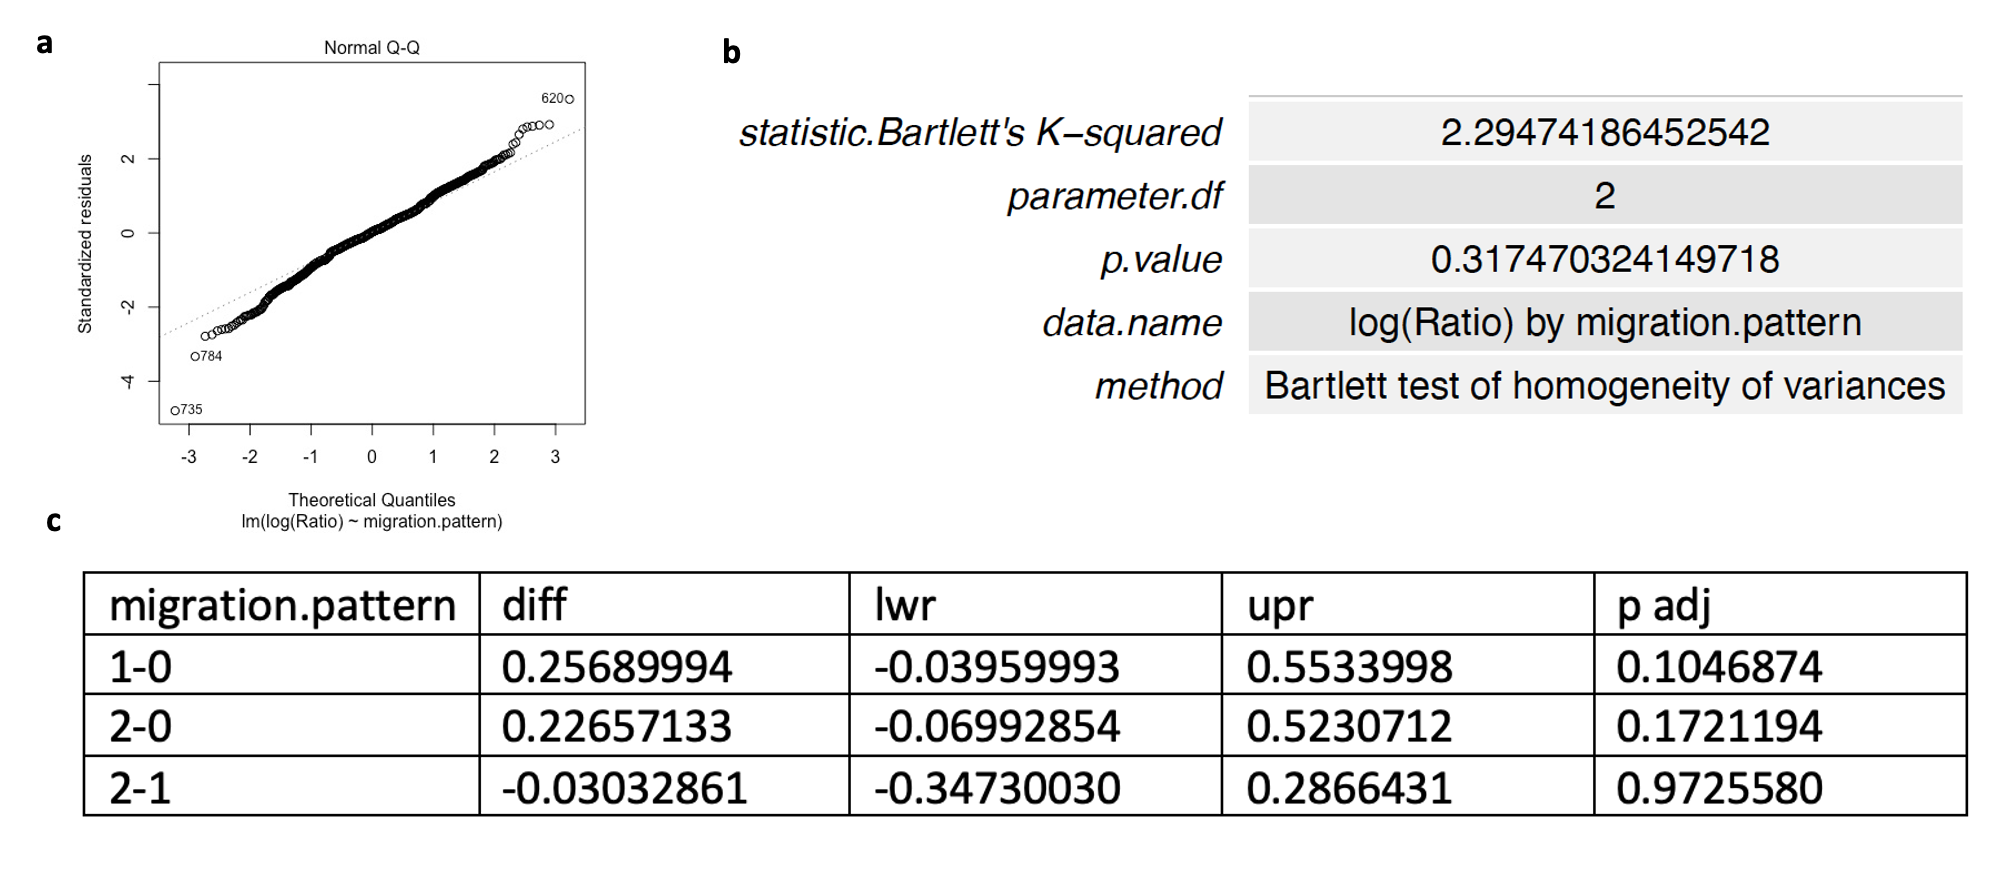
\includegraphics[width=0.9\textwidth]{../Results/anova_checks.jpg}
\end{figure}

\end{appendices}

\end{document}
